\documentclass[12pt]{amsart}

% PACKAGES
\usepackage{amsmath}
\usepackage{amssymb}
\usepackage{amsfonts}
\usepackage[alphabetic]{amsrefs}
\usepackage{amsthm}
% \usepackage{enumitem}
\usepackage{enumerate}
\usepackage{fullpage}
\usepackage{color}
\usepackage{graphicx}
\usepackage{wrapfig}
\usepackage{hyperref}
\usepackage{microtype,correctmathalign}
\usepackage{tikz}
\usepackage{float}
\usepackage{caption}
%\usepackage{quiver}
%\hypersetup{linktoc = all, colorlinks = true, urlcolor = Blue, linkcolor = Red, citecolor = RoyalBlue}
%\usepackage[parfill]{parskip}

% COMMANDS 
\newcommand{\nc}{\newcommand}
\newcommand{\rc}{\renewcommand}
\nc{\on}{\operatorname}

% EDITING
\definecolor{red}{rgb}{1,0,0}
\definecolor{orange}{rgb}{1,0.5,0}
\definecolor{purple}{rgb}{.5,.2,.8}
\definecolor{blue}{rgb}{.2,.2,.8}
\definecolor{green}{rgb}{.4,.6,.4}
\newcommand{\question}[1]{\noindent  \textcolor{red}{Question: #1}}
\newcommand{\todo}[1]{\noindent  \textcolor{blue}{To do: #1}}
% Editing line spacing
%\linespread{1.5}

% BLACKBOARD BOLD
\rc{\AA}{\mathbb{A}}	
\nc{\BB}{\mathbb{B}}	
\nc{\CC}{\mathbb{C}}	
\nc{\DD}{\mathbb{D}}	
\nc{\EE}{\mathbb{E}}	
\nc{\FF}{\mathbb{F}}	
\nc{\GG}{\mathbb{G}}	
\nc{\HH}{\mathbb{H}}	
\nc{\II}{\mathbb{I}}	
\nc{\JJ}{\mathbb{J}}	
\nc{\KK}{\mathbb{K}}	
\nc{\LL}{\mathbb{L}}	
\nc{\MM}{\mathbb{M}}	
\nc{\NN}{\mathbb{N}}	
\nc{\OO}{\mathbb{O}}	
\nc{\PP}{\mathbb{P}}	
\nc{\QQ}{\mathbb{Q}}	
\nc{\RR}{\mathbb{R}}	
\rc{\SS}{\mathbb{S}}	
\nc{\TT}{\mathbb{T}}	
\nc{\UU}{\mathbb{U}}	
\nc{\VV}{\mathbb{V}}	
\nc{\WW}{\mathbb{W}}	
\nc{\XX}{\mathbb{X}}	
\nc{\YY}{\mathbb{Y}}	
\nc{\ZZ}{\mathbb{Z}}	

% BOLD FACE
\nc{\bA}{\mathbf{A}}	
\nc{\bB}{\mathbf{B}}	
\nc{\bC}{\mathbf{C}}	
\nc{\bD}{\mathbf{D}}	
\nc{\bE}{\mathbf{E}}	
\nc{\bF}{\mathbf{F}}	
\nc{\bG}{\mathbf{G}}	
\nc{\bH}{\mathbf{H}}	
\nc{\bI}{\mathbf{I}}	
\nc{\bJ}{\mathbf{J}}	
\nc{\bK}{\mathbf{K}}	
\nc{\bL}{\mathbf{L}}	
\nc{\bM}{\mathbf{M}}	
\nc{\bN}{\mathbf{N}}	
\nc{\bO}{\mathbf{O}}	
\nc{\bP}{\mathbf{P}}	
\nc{\bQ}{\mathbf{Q}}	
\nc{\bR}{\mathbf{R}}	
\nc{\bS}{\mathbf{S}}	
\nc{\bT}{\mathbf{T}}	
\nc{\bU}{\mathbf{U}}	
\nc{\bV}{\mathbf{V}}	
\nc{\bW}{\mathbf{W}}	
\nc{\bX}{\mathbf{X}}	
\nc{\bY}{\mathbf{Y}}	
\nc{\bZ}{\mathbf{Z}}	

% CALLIGRAPHIC
\nc{\calA}{\mathcal{A}}	
\nc{\calB}{\mathcal{B}}	
\nc{\calC}{\mathcal{C}}	
\nc{\calD}{\mathcal{D}}	
\nc{\calE}{\mathcal{E}}	
\nc{\calF}{\mathcal{F}}	
\nc{\calG}{\mathcal{G}}	
\nc{\calH}{\mathcal{H}}	
\nc{\calI}{\mathcal{I}}	
\nc{\calJ}{\mathcal{J}}	
\nc{\calK}{\mathcal{K}}	
\nc{\calL}{\mathcal{L}}	
\nc{\calM}{\mathcal{M}}	
\nc{\calN}{\mathcal{N}}	
\nc{\calO}{\mathcal{O}}	
\nc{\calP}{\mathcal{P}}	
\nc{\calQ}{\mathcal{Q}}	
\nc{\calR}{\mathcal{R}}	
\nc{\calS}{\mathcal{S}}
\nc{\calT}{\mathcal{T}}	
\nc{\calU}{\mathcal{U}}	
\nc{\calV}{\mathcal{V}}	
\nc{\calW}{\mathcal{W}}
\nc{\calX}{\mathcal{X}}	
\nc{\calY}{\mathcal{Y}}	
\nc{\calZ}{\mathcal{Z}}

% LOWERCASE FRAK
\nc{\fraka}{\mathfrak{a}}
\nc{\frakb}{\mathfrak{b}}
\nc{\frakc}{\mathfrak{c}}
\nc{\frakd}{\mathfrak{d}}
\nc{\frake}{\mathfrak{e}}
\nc{\frakf}{\mathfrak{f}}
\nc{\frakg}{\mathfrak{g}}
\nc{\frakh}{\mathfrak{h}}
\nc{\fraki}{\mathfrak{i}}
\nc{\frakj}{\mathfrak{j}}
\nc{\frakk}{\mathfrak{k}}
\nc{\frakl}{\mathfrak{l}}
\nc{\frakm}{\mathfrak{m}}
\nc{\frakn}{\mathfrak{n}}
\nc{\frako}{\mathfrak{o}}
\nc{\frakp}{\mathfrak{p}}
\nc{\frakq}{\mathfrak{q}}
\nc{\frakr}{\mathfrak{r}}
\nc{\fraks}{\mathfrak{s}}
\nc{\frakt}{\mathfrak{t}}
\nc{\fraku}{\mathfrak{u}}
\nc{\frakv}{\mathfrak{v}}
\nc{\frakw}{\mathfrak{w}}
\nc{\frakx}{\mathfrak{x}}
\nc{\fraky}{\mathfrak{y}}
\nc{\frakz}{\mathfrak{z}}

% UPPERCASE FRAK
\nc{\frakA}{\mathfrak{A}}
\nc{\frakB}{\mathfrak{B}}
\nc{\frakC}{\mathfrak{C}}
\nc{\frakD}{\mathfrak{D}}
\nc{\frakE}{\mathfrak{E}}
\nc{\frakF}{\mathfrak{F}}
\nc{\frakG}{\mathfrak{G}}
\nc{\frakH}{\mathfrak{H}}
\nc{\frakI}{\mathfrak{I}}
\nc{\frakJ}{\mathfrak{J}}
\nc{\frakK}{\mathfrak{K}}
\nc{\frakL}{\mathfrak{L}}
\nc{\frakM}{\mathfrak{M}}
\nc{\frakN}{\mathfrak{N}}
\nc{\frakO}{\mathfrak{O}}
\nc{\frakP}{\mathfrak{P}}
\nc{\frakQ}{\mathfrak{Q}}
\nc{\frakR}{\mathfrak{R}}
\nc{\frakS}{\mathfrak{S}}
\nc{\frakT}{\mathfrak{T}}
\nc{\frakU}{\mathfrak{U}}
\nc{\frakV}{\mathfrak{V}}
\nc{\frakW}{\mathfrak{W}}
\nc{\frakX}{\mathfrak{X}}
\nc{\frakY}{\mathfrak{Y}}
\nc{\frakZ}{\mathfrak{Z}}

% OPERATORS
\nc{\Lie}{\on{Lie}}
\nc{\GL}{\on{GL}}
\nc{\PGL}{\on{PGL}}
\nc{\SL}{\on{SL}}
\nc{\Sp}{\on{Sp}}
\nc{\GSp}{\on{GSp}}
\nc{\SO}{\on{SO}}
\nc{\Or}{\on{O}}
\nc{\gl}{\on{\mathfrak{gl}}}
\rc{\sl}{\on{\mathfrak{sl}}}
\nc{\git}{/\!\!/}

\nc{\Mat}{\on{Mat}}
\nc{\Fun}{\on{Fun}}
\nc{\Aut}{\on{Aut}}
\nc{\End}{\on{End}}
\nc{\Hom}{\on{Hom}}
\nc{\Sym}{\on{Sym}}
\nc{\Span}{\on{span}}
\nc{\Irr}{\on{Irr}}
\nc{\Uch}{\on{Uch}}
\nc{\Type}{\on{Type}}
\nc{\Spec}{\on{Spec}}

\nc{\Ind}{\on{Ind}}
\nc{\Res}{\on{Res}}
\nc{\stab}{\on{stab}}
\nc{\orb}{\on{orb}}
\rc{\ker}{\on{ker}}
\nc{\im}{\on{im}}
\nc{\tr}{\on{tr}}
\nc{\ord}{\on{ord}}
\nc{\Tor}{\on{Tor}}
\nc{\Ad}{\on{Ad}}

\nc{\Id}{\on{Id}}
\nc{\Log}{\on{Log}}
\nc{\Exp}{\on{Exp}}
\nc{\Frac}{\on{Frac}}
\nc{\diag}{\on{diag}}
\nc{\D}{\on{D}}

% MATHRM
\nc{\St}{\mathrm{St}}
\nc{\triv}{\mathrm{triv}}
\nc{\sgn}{\mathrm{sgn}}
\nc{\reg}{\mathrm{reg}}
\nc{\rank}{\mathrm{rank}}
\nc{\op}{\mathrm{op}}
\nc{\ad}{\mathrm{ad}}
\rc{\ss}{\mathrm{ss}}
\nc{\HLV}{\mathrm{HLV}}

% ENVIRONMENTS
\theoremstyle{plain}
\newtheorem{theorem}{Theorem}%[subsection]
\newtheorem{definition}[theorem]{Definition}
\newtheorem{corollary}[theorem]{Corollary}
\newtheorem{lemma}[theorem]{Lemma}
\newtheorem{proposition}[theorem]{Proposition}
\newtheorem{claim}[theorem]{Claim}
\newtheorem{example}[theorem]{Example}
\newtheorem{remark}[theorem]{Remark}

% CONE PLOTTING
\usepackage{graphicx} % For including graphics
\usepackage{subcaption} % For subfigures
\usepackage{tikz}
\usepackage{amsmath}
\usepackage{pgfplots}
\pgfplotsset{compat=1.17}
\usepackage{tikz,tikz-3dplot}
\tdplotsetmaincoords{80}{45}
\tdplotsetrotatedcoords{-90}{180}{-90}

%% style for surfaces
\tikzset{surface/.style={draw=gray!70!black, fill=gray!40!white, fill opacity=.6}}

%% macros to draw back and front of cones
%% optional first argument is styling; others are z, radius, side offset (in degrees)
\newcommand{\coneback}[4][]{
  %% start at the correct point on the circle, draw the arc, then draw to the origin of the diagram, then close the path
  \draw[canvas is xy plane at z=#2, #1] (45-#4:#3) arc (45-#4:225+#4:#3) -- (O) --cycle;
}
\newcommand{\conefront}[4][]{
  \draw[canvas is xy plane at z=#2, #1] (45-#4:#3) arc (45-#4:-135+#4:#3) -- (O) --cycle;
}

\allowdisplaybreaks
%%%%%%%%%%%%%%%%%%%%%%%%%%%%%%%%%%%%%%%%%%%%%%%%%%%%%%%%%%%%%%%%%%%%%%%%%%%%%%%%
% The GIT quotient of a Lie algebra by a maximal torus, g // T
%%%%%%%%%%%%%%%%%%%%%%%%%%%%%%%%%%%%%%%%%%%%%%%%%%%%%%%%%%%%%%%%%%%%%%%%%%%%%%%%
\begin{document}
\section{The GIT quotient of a Lie algebra by a maximal torus, $\frakg \git T$}
\subsection{The $G=SL_3$ case}
Let $G = SL_3(\CC)$ and consider the adjoint action of $G$ on $\mathfrak{g} = \mathfrak{sl}_3(\CC)$.
A one-parameter subgroup $\lambda$ of $T$ is of the form
$$t \mapsto \begin{pmatrix} t^a & & \\ & t^b & \\ & & t^c \end{pmatrix}$$
for some $a, b, \in \mathbb{Z}$ and $a + b + c = 0$.
Composing with the adjoint action, we have
$$t 
\overset{\lambda}{\mapsto} \begin{pmatrix} t^a & & \\ & t^b & \\ & & t^c \end{pmatrix}
 \overset{\mathrm{Ad}}{\mapsto} \begin{pmatrix} v_{11} & t^{a-b} v_{12} & t^{2a+b} v_{13} \\ t^{-a+b} v_{21} & v_{22} & t^{a+2b} v_{23} \\ t^{-2a-b} v_{31} & t^{-a-2b} v_{32} & v_{33} \end{pmatrix}.$$
So the representation of $\CC^\times$ given by the composition $\mathrm{Ad} \circ \lambda: \CC^\times \to GL(\mathfrak{g})$ decomposes into the following weight spaces:
\begin{align*}
	\frakg &= \frakh \oplus \frakg_{\varepsilon_1} \oplus \frakg_{\varepsilon_2} \oplus \frakg_{\varepsilon_1 + \varepsilon_2} \oplus \frakg_{-\varepsilon_1} \oplus \frakg_{-\varepsilon_2} \oplus \frakg_{-\varepsilon_1 - \varepsilon_2}. 
\end{align*}
The respective weights are
$$0, \, a-b, \, a+2b, \, 2a+b, \, -a+b, \, -a-2b, \,-2a-b.$$
Here $\varepsilon_1(t) = t^{a-b}, \varepsilon_2(t) = t^{a+2b}$.

Let us say the weights of $v \in \frakg$ are the weights in which $v$ has a non-zero component.
The Hilbert-Mumford criterion gives us conditions for the stability of $v$ in terms of the weights of $v$:
\begin{enumerate}
\item $v \in \frakg$ is unstable if and only if there exists $\lambda \in X_*(T)\setminus\{0\}$ such that $v$ admits only positive or only negative weights.

\item $v \in \frakg$ is semi-stable if and only if for all $\lambda \in X_*(T)\setminus\{0\}$, $v$ admits both non-negative and non-positive weights.

\item $v \in \frakg$ is stable if and only if for all $\lambda \in X_*(T)\setminus\{0\}$, $v$ admits both positive and negative weights.
\end{enumerate}

\begin{example}
The vector 
$$v = \begin{pmatrix} 0 & 0 & 1 \\ 0 & 0 & 1 \\ 0 & 0 & 0 \end{pmatrix} \in \frakg_{\varepsilon_2} \oplus \frakg_{\varepsilon_1 + \varepsilon_2}$$
has weights $2a + b, a + 2b$.
When $a = b = -1$, $v$ admits only negative weights, so $v$ is unstable.

The vector 
$$v = \begin{pmatrix} 0 & 1 & 0 \\ 1 & 0 & 0 \\ 0 & 0 & 0 \end{pmatrix} \in \frakg_{\varepsilon_1} \oplus \frakg_{-\varepsilon_1}$$
has weights $a-b, - (a-b)$.
For all $a, b \in \mathbb{Z}$, one of the weights is non-negative and one is non-positive, so $v$ is semistable.
However, $v$ is not stable since $a=b=1$ gives a one-parameter subgroup where we do not have both positive and negative weights.

The vector 
$$v = \begin{pmatrix} 0 & 1 & 0 \\ 1 & 0 & 1 \\ 0 & 1 & 0 \end{pmatrix} \in  \frakg_{\varepsilon_1} \oplus \frakg_{-\varepsilon_1} \oplus  \frakg_{\varepsilon_2} \oplus \frakg_{-\varepsilon_2}$$
has weights $a-b, -(a-b), a+2b, -(a+2b)$.
For all $a, b \in \mathbb{Z}$, either $a-b, -(a-b)$ is a pair of positive and negative weights, or $a+2b, -(a+2b)$ is, so $v$ always has positive and negative weights.
Therefore, $v$ is stable.
\end{example}

\begin{example}
We list further examples of the stability of vectors in $\mathfrak{sl}_3$, which were checked using a computer.
The following vectors are unstable:
$$
\begin{pmatrix} 
	0 & 1 & 0 \\ 
	0 & 0 & 1 \\
	0 & 0 & 0 
\end{pmatrix}, \, 
\begin{pmatrix} 
	0 & 1 & 0 \\ 
	0 & 0 & 0 \\
	1 & 0 & 0 
\end{pmatrix}, \, 
\begin{pmatrix} 
	0 & 1 & 1 \\ 
	0 & 0 & 0 \\
	0 & 1 & 0 
\end{pmatrix}.
$$
It is interesting to note that these are all nilpotent matrices.
The following vectors are semi-stable and not stable:
$$
\begin{pmatrix} 
	0 & 1 & 0 \\ 
	1 & 0 & 1 \\
	0 & 0 & 0 
\end{pmatrix}, \, 
\begin{pmatrix} 
	0 & 0 & 0 \\ 
	0 & 0 & 1 \\
	0 & 1 & 0 
\end{pmatrix}, \, 
\begin{pmatrix} 
	0 & 1 & 1 \\ 
	0 & 0 & 1 \\
	0 & 1 & 0 
\end{pmatrix}.
$$
The following vectors are stable:
$$
\begin{pmatrix} 
	0 & 1 & 0 \\ 
	0 & 0 & 1 \\
	1 & 0 & 0 
\end{pmatrix}, \, 
\begin{pmatrix} 
	0 & 1 & 0 \\ 
	1 & 0 & 1 \\
	0 & 1 & 0 
\end{pmatrix}, \, 
\begin{pmatrix} 
	0 & 1 & 1 \\ 
	1 & 0 & 0 \\
	1 & 0 & 0 
\end{pmatrix}.
$$ \\
\end{example}

\subsection{The $G = Sp_4$ case}
Now let $G = Sp_4(\CC)$ and $\mathfrak{g} = \mathfrak{sp}_4(\CC)$.
Composing a one-parameter subgroup of $T$ with the adjoint action gives a map
$$t 
\overset{\lambda}{\mapsto} 
\begin{pmatrix} 
	t^a & & & \\ 
	& t^b & & \\ 
	& & t^{-b} & \\
	& & & t^{-a} 
\end{pmatrix}
\overset{\mathrm{Ad}}{\mapsto} 
\begin{pmatrix} 
	v_{11} & t^{a-b} v_{12} & t^{a+b} v_{13} & t^{2a} v_{14} \\ 
	t^{-(a-b)} v_{21} & v_{22} & t^{2b} v_{23} & t^{a+b} v_{24} \\ 
	t^{-(a+b)} v_{31} & t^{-2b} v_{32} & v_{33} & t^{a-b} v_{34} \\
	t^{-2a} v_{41} & t^{-(a+b)} v_{42} & t^{-(a-b)} v_{43} & v_{44}
\end{pmatrix},$$
where $a, b \in \mathbb{Z}$.
So the representation $\mathrm{Ad} \circ \lambda : \CC^\times \to \mathfrak{sp}_4$ decomposes as
$$
\mathfrak{g} 
= \frakh \oplus \frakg_{\varepsilon_1-\varepsilon_2} \oplus \frakg_{2 \varepsilon_2} \oplus \frakg_{\varepsilon_1+\varepsilon_2} \oplus \frakg_{2\varepsilon_1} 
\oplus \frakg_{-(\varepsilon_1-\varepsilon_2)} \oplus \frakg_{-2 \varepsilon_2} \oplus \frakg_{-(\varepsilon_1+\varepsilon_2)} \oplus \frakg_{-2\varepsilon_1}, 
$$
where the respective weights are
$$0, \,\, a-b, \,\, 2b, \,\, a+b, \,\, 2a, \,\, -(a-b), \,\, -2b, \,\, -(a+b), \,\, -2a.$$
Here $\varepsilon_1(t) = t^{a}$, $\varepsilon_2(t) = t^{b}$.

\begin{example}
The vector 
$$v = 
\begin{pmatrix}
	0 & 1 & 0 & 0 \\
	0 & 0 & 1 & 0 \\
	0 & 0 & 0 & 1 \\
	0 & 0 & 0 & 0 
\end{pmatrix} \in \frakg_{\varepsilon_1 - \varepsilon_2} \oplus \frakg_{2 \varepsilon_2}
$$
has weights $a-b, 2b$.
When $a = -2, b = -1$, $v$ admits only negative weights, so $v$ is unstable.

The vector 
$$v = 
\begin{pmatrix}
	0 & 1 & 0 & 0 \\
	1 & 0 & 0 & 0 \\
	0 & 0 & 0 & 1 \\
	0 & 0 & 1 & 0 
\end{pmatrix} \in \frakg_{\varepsilon_1 - \varepsilon_2} \oplus \frakg_{-(\varepsilon_1 -  \varepsilon_2)}
$$
has weights $a-b, -(a-b)$, which always has a non-negative and non-positive weight for all $a, b \in \mathbb{Z}$, so $v$ is semi-stable.
When $a=b=1$, we do not have a positive and negative weight, so $v$ is not stable.

The vector
$$v = 
\begin{pmatrix}
	0 & 1 & 0 & 0 \\
	1 & 0 & 1 & 0 \\
	0 & 1 & 0 & 1 \\
	0 & 0 & 1 & 0 
\end{pmatrix} \in \frakg_{\varepsilon_1 - \varepsilon_2} \oplus \frakg_{2 \varepsilon_2} \oplus \frakg_{-(\varepsilon_1 -  \varepsilon_2)} \oplus \frakg_{- 2\varepsilon_2} 
$$
has weights $a-b, 2b, -(a-b), -2b$, which contains positive and negative weights for all $a, b \in \mathbb{Z}$.
Therefore, $v$ is stable.
\end{example}

\begin{example}
The following examples of stability for vectors in $\mathfrak{sp}_4$ were checked using a computer.
The following vectors are unstable:
$$
\begin{pmatrix} 
	0 & 1 & 0 & 0 \\ 
	0 & 0 & 0 & 0 \\
	0 & 1 & 0 & 1 \\
	0 & 0 & 0 & 0
\end{pmatrix}, \, 
\begin{pmatrix} 
	0 & 0 & 0 & 0 \\ 
	0 & 0 & 1 & 0 \\
	1 & 0 & 0 & 0 \\
	0 & -1 & 0 & 0
\end{pmatrix}, \, 
\begin{pmatrix} 
	0 & 0 & 0 & 0 \\ 
	1 & 0 & 1 & 0 \\
	1 & 0 & 0 & 0 \\
	0 & -1 & 1 & 0
\end{pmatrix}.
$$
It is interesting to note that these are all nilpotent matrices.
The following vectors are semi-stable and not stable:
$$
\begin{pmatrix} 
	0 & 0 & 0 & 0 \\ 
	0 & 0 & 1 & 0 \\
	0 & 1 & 0 & 0 \\
	0 & 0 & 0 & 0
\end{pmatrix}, \, 
\begin{pmatrix} 
	0 & 0 & 0 & 0 \\ 
	1 & 0 & 1 & 0 \\
	0 & 1 & 0 & 0 \\
	0 & 0 & 1 & 0
\end{pmatrix}, \, 
\begin{pmatrix} 
	0 & 1 & 1 & 1 \\ 
	0 & 0 & 0 & -1 \\
	1 & 0 & 0 & 1 \\
	0 & -1 & 0 & 0
\end{pmatrix}.
$$
The following vectors are stable:
$$
\begin{pmatrix} 
	0 & 0 & 1 & 0 \\ 
	1 & 0 & 0 & -1 \\
	0 & 1 & 0 & 0 \\
	0 & 0 & 1 & 0
\end{pmatrix}, \,
\begin{pmatrix} 
	0 & 0 & 1 & 0 \\ 
	0 & 0 & 0 & -1 \\
	0 & 1 & 0 & 0 \\
	1 & 0 & 0 & 0
\end{pmatrix}, \, 
\begin{pmatrix} 
	0 & 0 & 0 & 1 \\ 
	1 & 0 & 0 & 0 \\
	0 & 1 & 0 & 0 \\
	0 & 0 & 1 & 0
\end{pmatrix}.
$$ 
\end{example}
%We have
%$$
%\begin{pmatrix} 
%	0 & 0 & 1 & 0 \\ 
%	0 & 0 & 0 & -1 \\
%	0 & 1 & 0 & 0 \\
%	1 & 0 & 0 & 0
%\end{pmatrix} \in \frakg_{\varepsilon_1+\varepsilon_2} \oplus \frakg_{-2\varepsilon_2} \oplus \frakg_{-2\varepsilon_1}$$
%with weights $a+b, -2b, -a$ and 
%$$
%\begin{pmatrix} 
%	0 & 0 & 0 & 1 \\ 
%	1 & 0 & 0 & 0 \\
%	0 & 1 & 0 & 0 \\
%	0 & 0 & 1 & 0
%\end{pmatrix} \in \frakg_{2\varepsilon_1} \oplus \frakg_{-(\varepsilon_1 - \varepsilon_2)} \oplus \frakg_{-2\varepsilon_2}$$
%with weights $2a, -(a-b), -2b$.

\subsection{The general case}
Let $G$ be a connected complex reductive group, $\frakg$ the Lie algebra and $T$ a maximal torus.
We are interested in the adjoint action of $T$ on $\frakg$.

Choose $x_\alpha \in \frakg_\alpha$ for each $\alpha \in \Phi$ such that $x_\alpha$ is a basis for $\frakg_\alpha$.
For any $x \in \frakg$, we can write
$$x = x_0 + \sum_{\alpha \in \Phi} k_\alpha x_\alpha, \qquad k_\alpha \in \CC.$$
Denote
$$S_x = \{\alpha \in \Phi \, | \, k_\alpha \ne 0\} \subseteq \Phi.$$

The list of examples leads to the following claim:

\begin{claim}
Let $x \in \frakg$.
Then:
\begin{enumerate}%[label=(\roman*)]
\item
$x$ is unstable if and only if for all $Z \subseteq S_x$ and for all coefficients $\{n_\alpha \in \ZZ_{>0} \, | \, \alpha \in Z\}$, 
$$\sum_{\alpha \in Z} n_\alpha \alpha \ne 0;$$

\item
$x$ is stable if and only if there exists $Z \subseteq S_x$ and coefficients $\{n_\alpha \in \ZZ_{>0} \, | \, \alpha \in Z\}$, with $|Z|$ sufficiently large, such that
$$\sum_{\alpha \in Z} n_\alpha \alpha = 0.$$
\end{enumerate}
\end{claim}

The exact meaning of what ``$|Z|$ sufficiently large'' should be is to be determined, for example, $|Z| > \mathrm{rank}(T)$.

For the [$\implies$] direction of (i), suppose $x$ is unstable and $S_x = \{\alpha_1, \ldots, \alpha_m\}$.
The Hilbert-Mumford criterion tells us that there exists $\lambda \in X_*(T)$ such that 
$$\langle \lambda, \alpha_1 \rangle, \ldots, \langle \lambda, \alpha_r \rangle > 0.$$
Then for all $Z \subseteq S_x$ and for all coefficients $\{n_\alpha \in \ZZ_{>0} \, | \, \alpha \in Z\}$,
$$\left\langle\lambda, \sum_{\alpha \in Z}  n_\alpha  \alpha \right \rangle
= \sum_{\alpha \in Z} n_\alpha  \langle \lambda, \alpha \rangle > 0 \implies \sum_{\alpha \in Z}  n_\alpha  \alpha \ne 0$$

The converse statement needed to prove (i) would be: 
suppose that for all $Z \subseteq S_x$ and all coefficients $\{n_\alpha \, | \, \alpha \in Z\}$, that $\sum_{\alpha \in Z} n_\alpha \alpha \ne 0$; to see $x$ is unstable, by Hilbert-Mumford we need to show that there exists $\lambda \in X_*(T)$ such that $\langle \lambda, \alpha \rangle > 0$ for all $\alpha_i \in Z$.
The contrapositive is: 
let $x$ be semi-stable, such that for all $\lambda \in X_*(T)$, there exist $\alpha_i, \alpha_j \in S_x$ so that $\langle \lambda, \alpha_i \rangle \le 0, \langle \lambda, \alpha_j \rangle \ge 0$; 
we need to show that there exist coefficients $\{n_\alpha \in \mathbb{Z}_{>0} \, | \, \alpha \in Z\}$ such that 
$$\sum_{\alpha \in \ZZ} n_\alpha \alpha = 0.$$

\subsection{The ring of invariants}
Recall that the algebra of polynomial functions on $\frakg$ can be thought of as the symmetric algebra $S(\frakg^*)$.
After fixing a basis for $\frakg$, there is the corresponding dual basis for $\frakg^*$ that gives a set of generators for $S(\frakg^*)$.
In particular, let $\frakh$ be a Cartan subalgebra of $\frakg$ and 
$$\{e_\alpha \, | \, \alpha \in \Phi\}\cup\{h_i \, | \, i=1,\ldots, r\}$$
a corresponding Cartan-Weyl basis for $\frakg$.
Let $\{x_\alpha\,|\,\alpha\in\Phi\}\cup\{y_i\,|\,i=1,\ldots,r\}\subseteq\frakg^*$ be the dual basis.
For $\eta = (\eta_\alpha)_{\alpha\in\Phi} \in (\ZZ_{\ge0})^{|\Phi|}, \mu = (\mu_1, \ldots, \mu_r)\in (\ZZ_{\ge0})^r$, denote
$$X^\eta = \prod_{\alpha\in\Phi} x_{\alpha}^{\eta_\alpha}, \qquad Y^\mu = \prod_{j=1}^r y_i^{\mu_j},$$
such that the set of monomials $\{X^\eta Y^\mu\,|\,\eta \in (\ZZ_{\ge0})^{|\Phi|}, \mu\in(\ZZ_{\ge0})^r\}$ are a basis for $S(\frakg^*)$.
We will write elements of $S(\frakg^*)$ as 
$$p = \sum_{(\eta, \mu)} p_{\eta,\mu} X^\eta Y^\mu, \qquad p_{\eta,\mu} \in \CC,$$
with the understanding that the sum is over finitely many exponents $(\eta, \mu)$.
Recall that $t \in T$ acts on $x \in \frakg$ by
$$t \cdot x = t \cdot \left(\sum_{\alpha\in\Phi} x_\alpha e_\alpha + \sum_{i=1}^r y_i h_i \right) = \sum_{\alpha\in\Phi} \alpha(t) x_\alpha e_\alpha + \sum_{i=1}^r y_i h_i,$$
implying $t \in T$ acts on the generator $x_\alpha \in S(\frakg^*)$ by
$$(t\cdot x_\alpha)(x) = x_\alpha(t^{-1} \cdot x) = \alpha(t^{-1}) x_\alpha = (-\alpha)(t) x_\alpha.$$
It follows that 
$$t \cdot p = \sum_{(\eta, \mu)} p_{\eta,\mu} \left(\sum_{\alpha\in\Phi} (- \eta_\alpha \alpha)(t)\right) X^\eta Y^\mu,$$
since roots are written additively, i.e., $(-\alpha(t))^{\eta_\alpha} = (-\eta_\alpha \alpha)(t)$

We want to understand the structure of $\CC[\frakg]^T$ in root-theoretic terms.
\begin{lemma}
A polynomial $p \in S(\frakg^*)$ is invariant if and only if for each monomial $X^\eta Y^\mu$ in $p$, it holds that
$$\sum_{\alpha\in\eta} \eta_\alpha \alpha = 0.$$
\end{lemma}
\begin{proof}
    By definition, $p \in S(\frakg^*)$ is invariant if for all $t \in T$,
    $$t\cdot p = \sum_{(\eta, \mu)} p_{\eta,\mu} \left(\sum_{\alpha\in\Phi} (- \eta_\alpha \alpha)(t)\right) X^\eta Y^\mu = \sum_{(\eta, \mu)} p_{\eta,\mu} X^\eta Y^\mu=p.$$
    But since the monomials $X^\eta Y^\mu$ are a basis for $S(\frakg^*)$, this equality is equivalent to having 
    $$\sum_{\alpha\in\Phi} (- \eta_\alpha \alpha)(t) = 1 \, \iff \, \sum_{\alpha\in\Phi} \eta_\alpha \alpha = 0$$
    for all $t \in T$ and every monomial $X^\eta Y^\mu$ in $p$.
\end{proof}

The lemma implies the following theorem.

\begin{theorem}
    The ring of invariants is
    $$\CC[\frakg]^T = \CC\left[X^\eta, Y^\mu \, \Big| \, \eta \in (\ZZ_{\ge0})^{|\Phi|}, \,\sum_{\alpha\in\Phi} \eta_\alpha \alpha = 0, \, \mu \in (\ZZ_{\ge0})^r\right].$$
\end{theorem}

To give a presentation of $\CC[\frakg]^T$ by generators and relations, we need to understand all the ways one can choose $\eta \in (\ZZ_{\ge0})^{|\Phi|}$ such that
$$\sum_{\alpha \in \Phi} \eta_\alpha \alpha = 0.$$

\subsection{Admissible and simple exponents}
With the goal of giving a presentation of $\CC[\frakg]^T$ by generators and relations in mind, in this section we will study exponents of monomials which we will call \emph{admissible}.

\begin{definition}
    An exponent $\eta \in (\ZZ_{\ge 0})^{|\Phi|}$ is \emph{admissible} if
    $$\sum_{\alpha \in \Phi} \eta_\alpha \alpha = 0.$$
\end{definition}

Observe that the sum of admissible exponents is admissible.
Finding generators for $\CC[\frakg]^T$ amounts to finding a minimal set of admissible exponents such that any admissible $\nu \in (\ZZ_{\ge0})^{|\Phi|}$ can be expressed as a sum of the minimal generating set.
The right notion of ``minimal" is essentially that an exponent cannot be expressed as a sum of other coefficients.

Introduce a partial order $\preceq$ on the set of exponents by declaring $\mu \preceq \eta$ if $\mu_\alpha \le \eta_\alpha$ for all $\alpha \in \Phi$.
Also, define the \emph{height} of an exponent by $\mathrm{ht}(\eta)=\sum_{\alpha\in\Phi} \eta_\alpha$.

\begin{definition}
An exponent $\eta \in (\ZZ_{\ge 0})^{|\Phi|}$ is called \emph{irreducible} if, whenever $\eta = \mu + \nu$ for admissible exponents $\mu$ and $\nu$, either $\mu=0$ or $\nu=0$. An exponent is reducible if it is not irreducible.
\end{definition}

\begin{example}
    Consider the $A_1$ root system $\Phi=\{\alpha,-\alpha\}$.
    The exponent $\eta=(\eta_\alpha, \eta_{-\alpha}) = (1, 1)$ is admissible and irreducible.
    The exponent $\nu=(\nu_\alpha, \nu_{-\alpha}) = (2, 2)$ is admissible but reducible, since $\nu = \eta + \eta$ and $\eta$ is admissible and nonzero.
\end{example}

\begin{proposition}
    Any exponent is a sum of irreducible exponents.
\end{proposition}
\begin{proof}
    \todo{write this out.}
\end{proof}

Our goal from here is to give a description of the simple admissible coefficients.

\begin{example}
For rank 2 root systems, we can denote admissible exponents by drawing the roots with nonzero component in red, scaled by the component corresponding to that root.
For example, if we consider the $A_2$ root system labelled with the following choice of simple roots $\{\alpha, \beta\}$

%\centerline{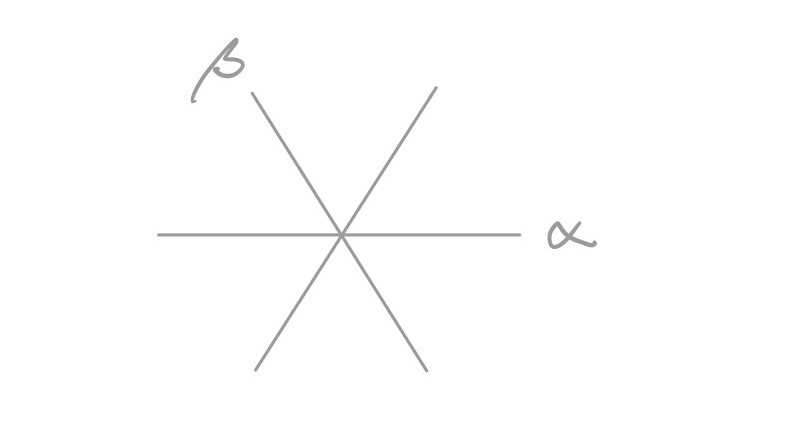
\includegraphics[scale=0.3]{A_2 root system.jpg}}

\noindent
We denote the admissible exponents $\eta, \nu$, where $\eta_{\alpha+\beta}, \eta_{-(\alpha+\beta)}=1$ and $\nu_{\alpha}, \nu_{-\alpha}=2$ and all other components zero, by

%\centerline{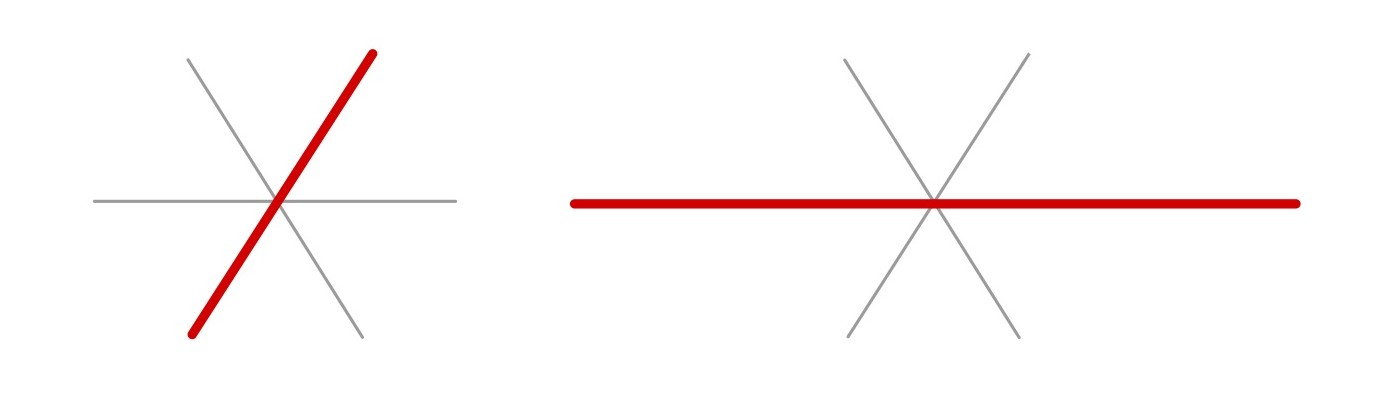
\includegraphics[scale=0.3]{A_2 diagram notation example.jpg}}

\noindent
We claim that the following is the complete set of simple admissible exponents for $A_2$ 
(it is straightforward to check these are all admissible and simple, though it is not obvious whether this is a complete set):

%\centerline{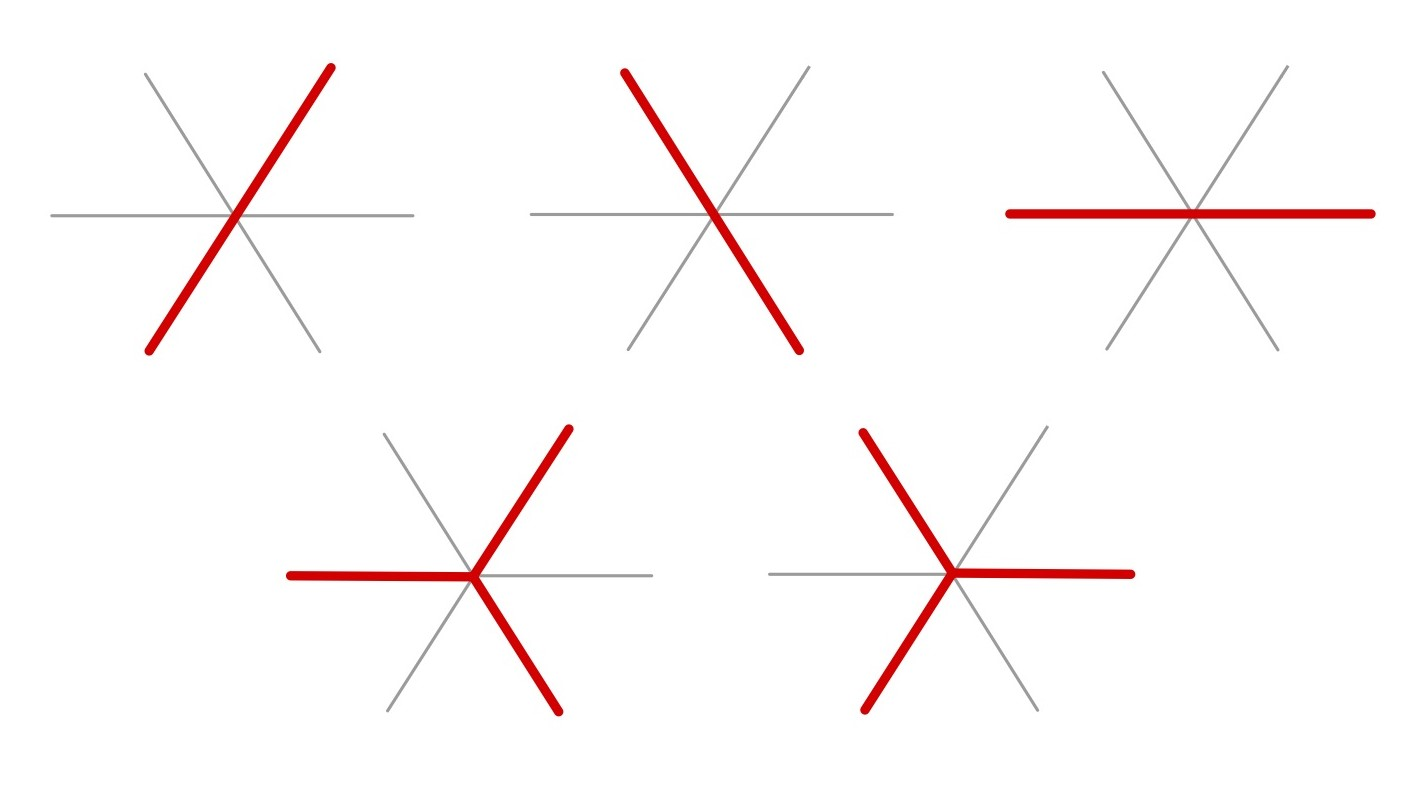
\includegraphics[scale=0.3]{A_2 simple admissibles.jpg}}

\noindent
If we consider the $C_2$ root system with the following choice of simple roots

%\centerline{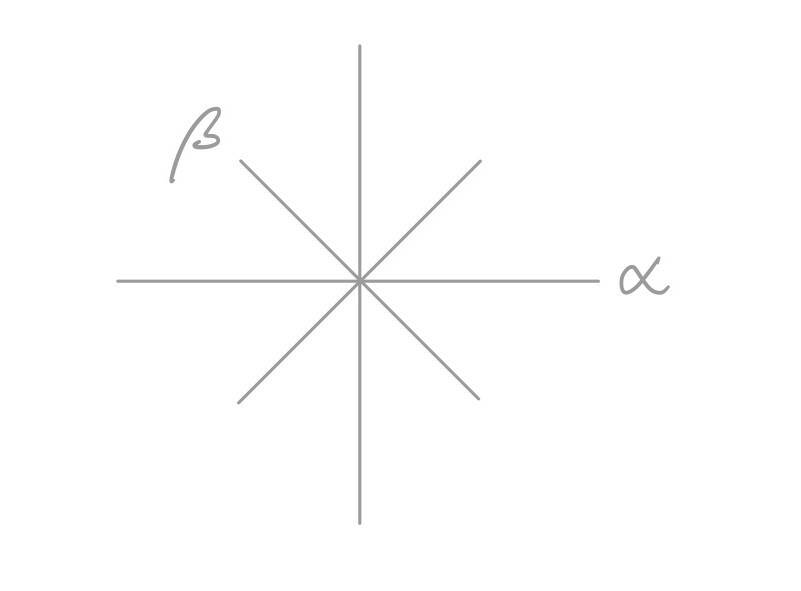
\includegraphics[scale=0.3]{C_2 root system.jpg}}

\noindent
Then we claim the following is the complete set of simple admissible exponents for $C_2$:

%\centerline{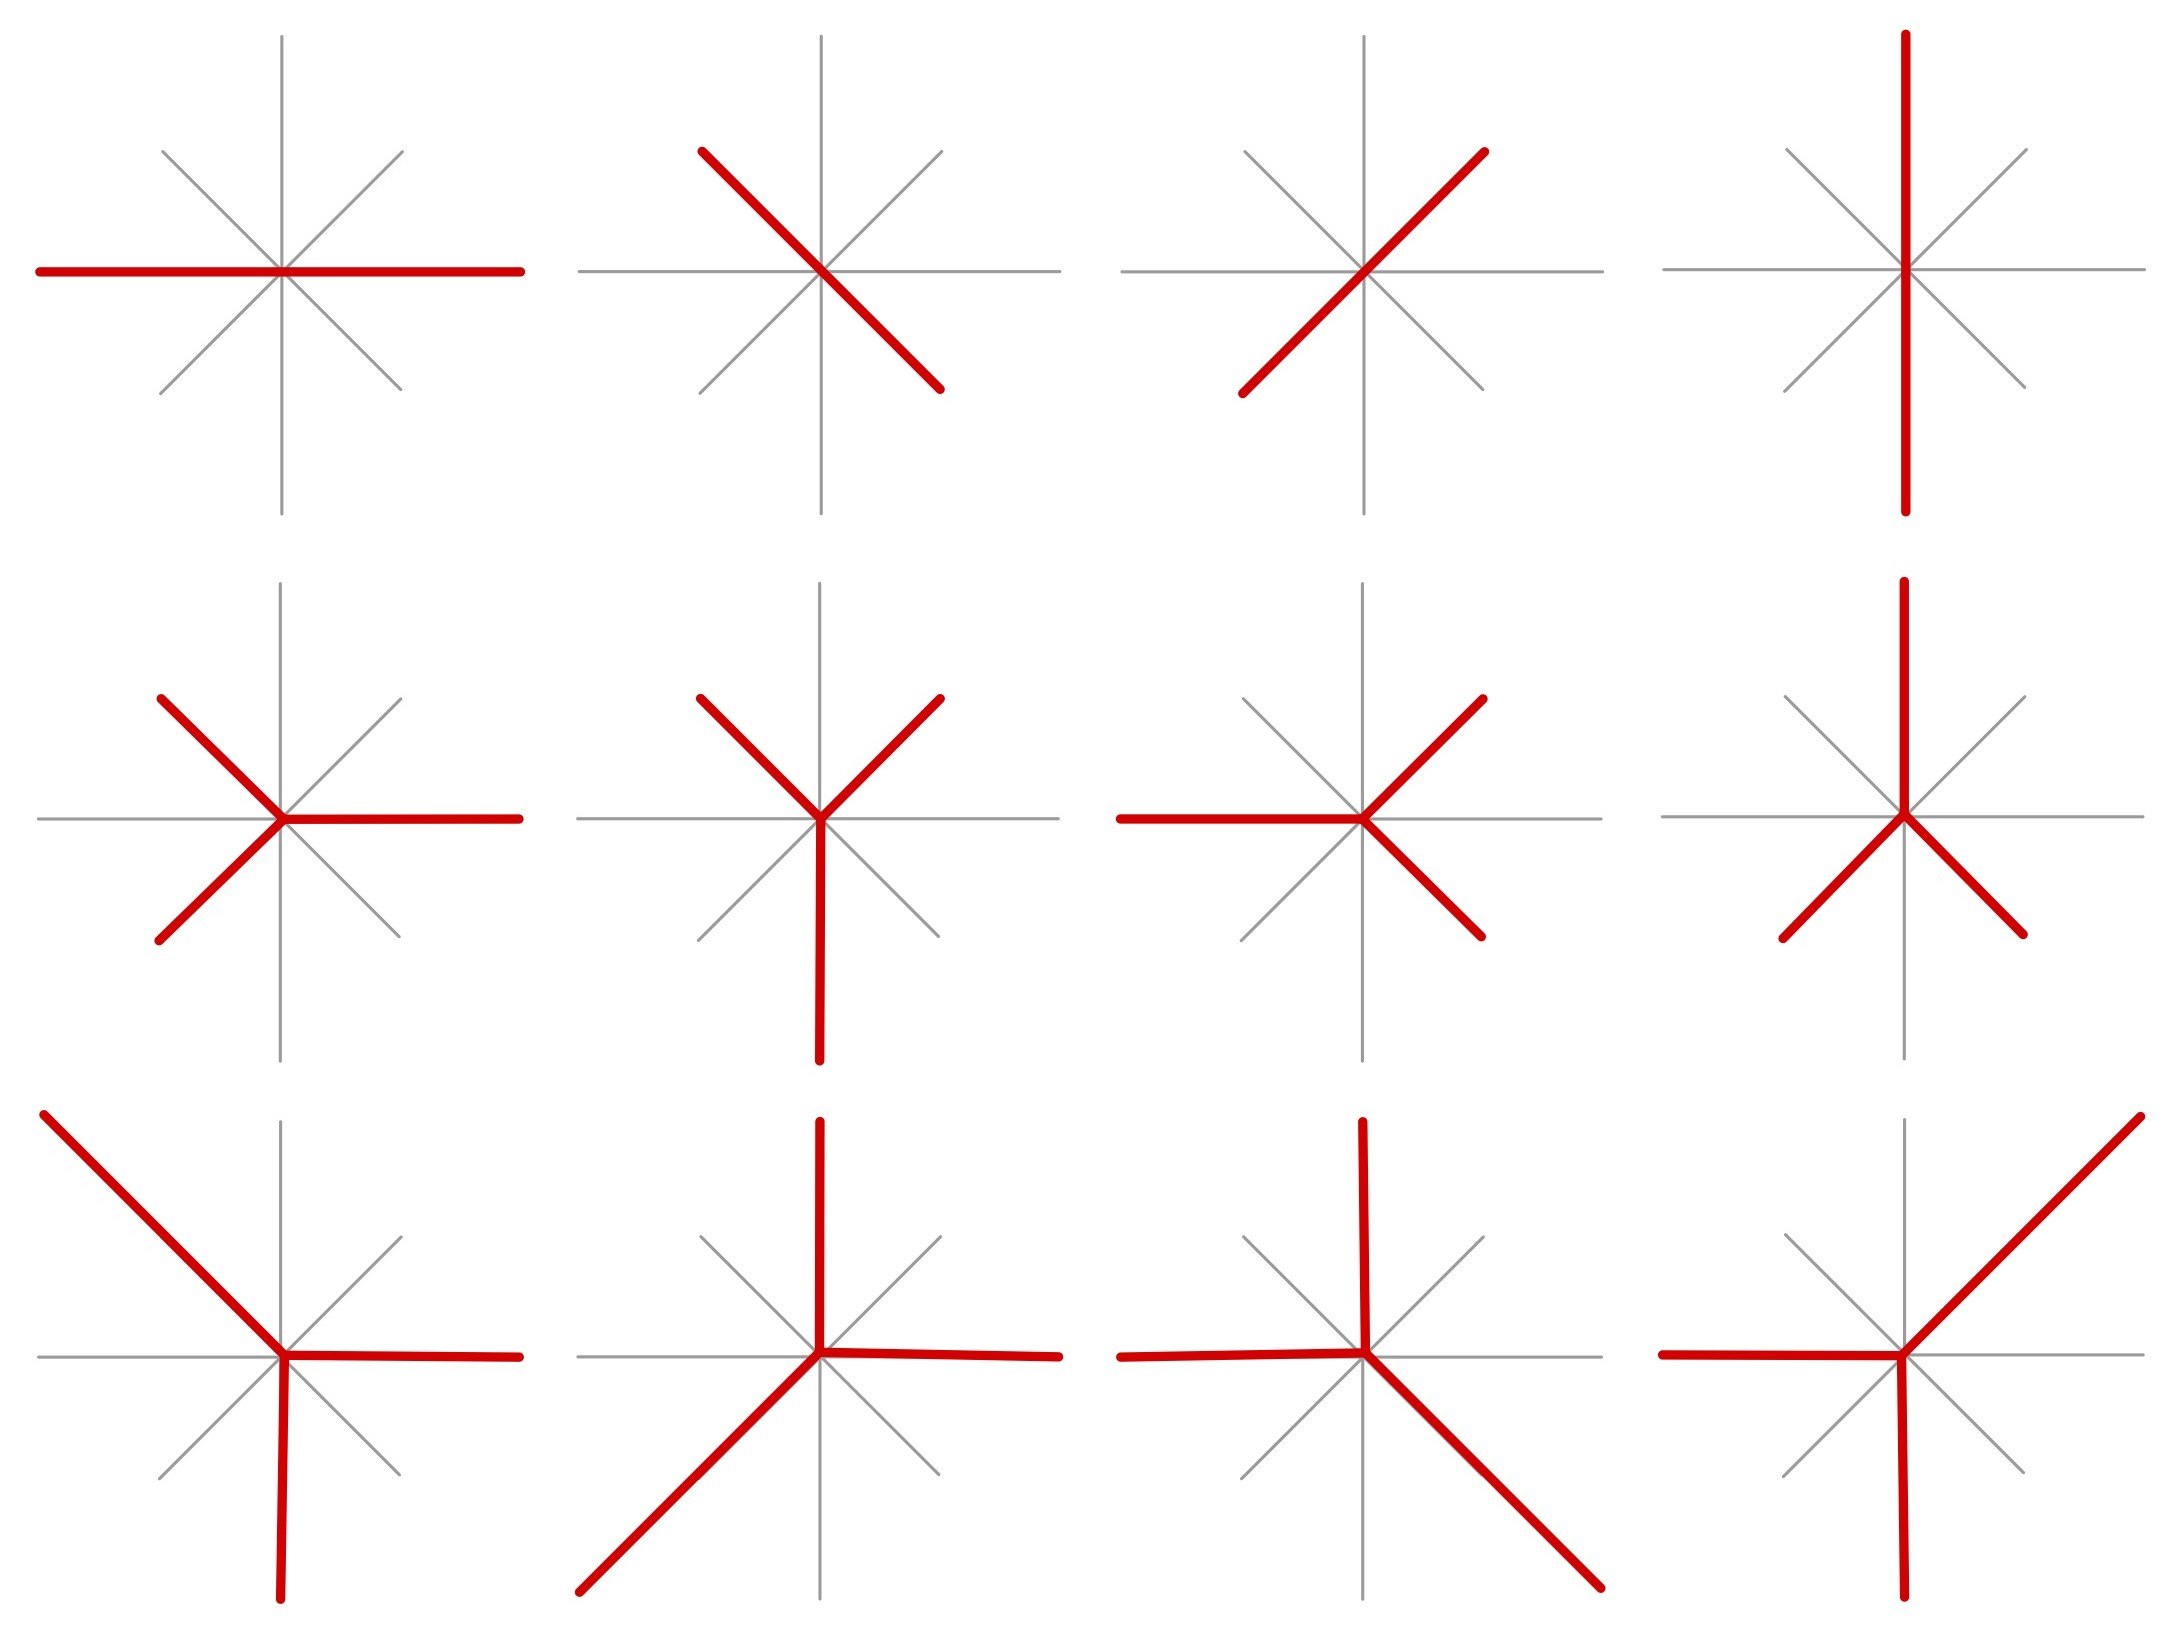
\includegraphics[scale=0.2]{C_2 simple admissibles.jpg}}

\end{example}
\end{document}